\documentclass[a4paper]{article}
\usepackage[margin=1cm]{geometry}
\usepackage{amsmath, amssymb}
\usepackage{graphicx}
\usepackage{tikz}
\usetikzlibrary{arrows.meta}
\pagestyle{empty}

\definecolor{c0}{HTML}{E53935}
\definecolor{c1}{HTML}{1E88E5}
\definecolor{c2}{HTML}{43A047}
\definecolor{c3}{HTML}{FB8C00}
\definecolor{c4}{HTML}{8E24AA}
\definecolor{c5}{HTML}{00ACC1}
\definecolor{c6}{HTML}{F4511E}
\definecolor{c7}{HTML}{3949AB}
\definecolor{c8}{HTML}{7CB342}
\definecolor{c9}{HTML}{C2185B}
\definecolor{c10}{HTML}{FF7043}
\definecolor{c11}{HTML}{26A69A}
\definecolor{c12}{HTML}{5C6BC0}
\definecolor{c13}{HTML}{FFCA28}
\definecolor{c14}{HTML}{AB47BC}

\begin{document}

\begin{center}
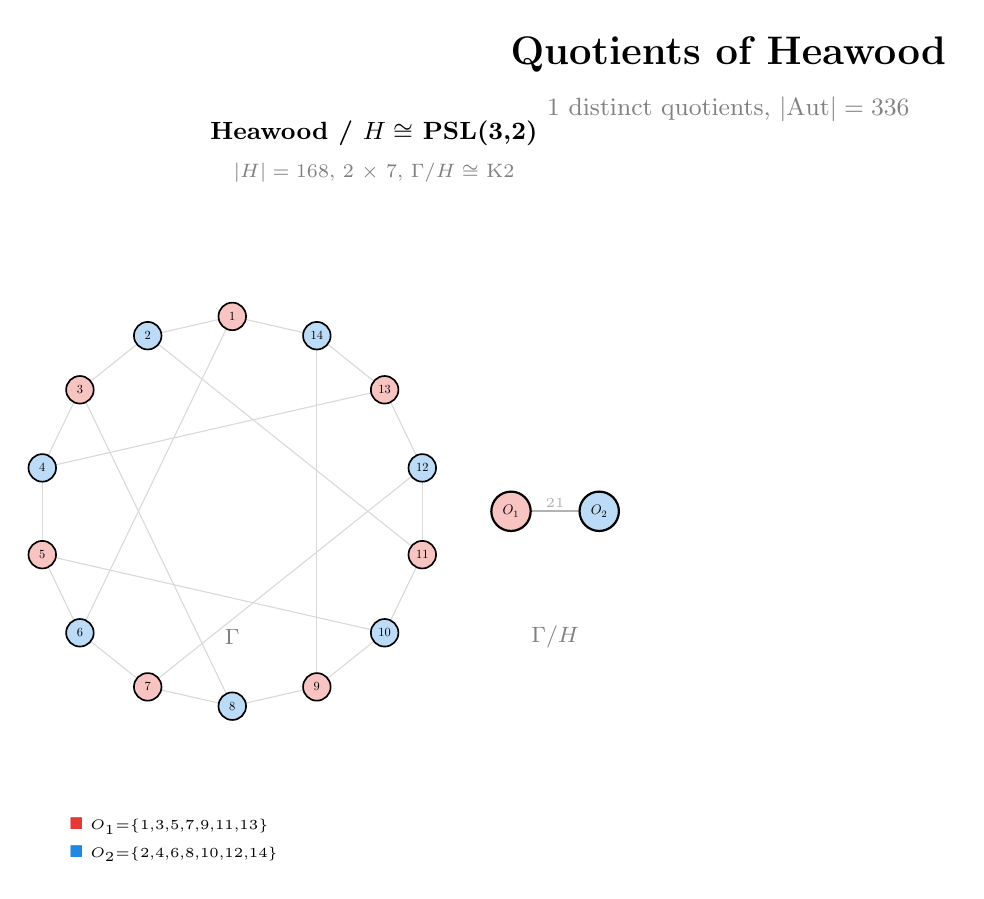
\begin{tikzpicture}[
  ov/.style={circle, draw, semithick, minimum size=3.5mm, inner sep=0pt},
  ovs/.style={circle, draw, thin, minimum size=1.8mm, inner sep=0pt},
  qv/.style={circle, draw, thick, minimum size=5mm, inner sep=0pt},
  cardtitle/.style={font=\small\bfseries},
  cardsub/.style={font=\scriptsize, text=gray},
  glabel/.style={font=\footnotesize, text=gray},
]
\node[font=\Large\bfseries] at (0, 11.5) {Quotients of Heawood};
\node[font=\small, text=gray] at (0, 10.8) {1 distinct quotients, $|\mathrm{Aut}|=336$};

% Card 1: H=PSL(3,2)
\node[cardtitle] at (-4.50,10.50) {Heawood / $H \cong$ PSL(3,2)};
\node[cardsub] at (-4.50,10.00) {$|H|=168$, 2 $\times$ 7, $\Gamma/H \cong$ K2};
\draw[gray!30, thin] (-6.300,8.175) -- (-7.374,7.930);
\draw[gray!30, thin] (-6.300,8.175) -- (-8.235,4.157);
\draw[gray!30, thin] (-6.300,8.175) -- (-5.226,7.930);
\draw[gray!30, thin] (-7.374,7.930) -- (-8.235,7.243);
\draw[gray!30, thin] (-7.374,7.930) -- (-3.887,5.149);
\draw[gray!30, thin] (-8.235,7.243) -- (-8.713,6.251);
\draw[gray!30, thin] (-8.235,7.243) -- (-6.300,3.225);
\draw[gray!30, thin] (-8.713,6.251) -- (-8.713,5.149);
\draw[gray!30, thin] (-8.713,6.251) -- (-4.365,7.243);
\draw[gray!30, thin] (-8.713,5.149) -- (-8.235,4.157);
\draw[gray!30, thin] (-8.713,5.149) -- (-4.365,4.157);
\draw[gray!30, thin] (-8.235,4.157) -- (-7.374,3.470);
\draw[gray!30, thin] (-7.374,3.470) -- (-6.300,3.225);
\draw[gray!30, thin] (-7.374,3.470) -- (-3.887,6.251);
\draw[gray!30, thin] (-6.300,3.225) -- (-5.226,3.470);
\draw[gray!30, thin] (-5.226,3.470) -- (-4.365,4.157);
\draw[gray!30, thin] (-5.226,3.470) -- (-5.226,7.930);
\draw[gray!30, thin] (-4.365,4.157) -- (-3.887,5.149);
\draw[gray!30, thin] (-3.887,5.149) -- (-3.887,6.251);
\draw[gray!30, thin] (-3.887,6.251) -- (-4.365,7.243);
\draw[gray!30, thin] (-4.365,7.243) -- (-5.226,7.930);
\node[ov, fill=c0!30] at (-6.300,8.175) {\scalebox{0.45}{1}};
\node[ov, fill=c1!30] at (-7.374,7.930) {\scalebox{0.45}{2}};
\node[ov, fill=c0!30] at (-8.235,7.243) {\scalebox{0.45}{3}};
\node[ov, fill=c1!30] at (-8.713,6.251) {\scalebox{0.45}{4}};
\node[ov, fill=c0!30] at (-8.713,5.149) {\scalebox{0.45}{5}};
\node[ov, fill=c1!30] at (-8.235,4.157) {\scalebox{0.45}{6}};
\node[ov, fill=c0!30] at (-7.374,3.470) {\scalebox{0.45}{7}};
\node[ov, fill=c1!30] at (-6.300,3.225) {\scalebox{0.45}{8}};
\node[ov, fill=c0!30] at (-5.226,3.470) {\scalebox{0.45}{9}};
\node[ov, fill=c1!30] at (-4.365,4.157) {\scalebox{0.45}{10}};
\node[ov, fill=c0!30] at (-3.887,5.149) {\scalebox{0.45}{11}};
\node[ov, fill=c1!30] at (-3.887,6.251) {\scalebox{0.45}{12}};
\node[ov, fill=c0!30] at (-4.365,7.243) {\scalebox{0.45}{13}};
\node[ov, fill=c1!30] at (-5.226,7.930) {\scalebox{0.45}{14}};
\node[glabel] at (-6.30,4.10) {$\Gamma$};
\node[qv, fill=c0!30] (c0o0) at (-2.760,5.700) {\scalebox{0.5}{$O_{1}$}};
\node[qv, fill=c1!30] (c0o1) at (-1.640,5.700) {\scalebox{0.5}{$O_{2}$}};
\draw[gray!60, thick] (c0o0) -- node[font=\tiny, auto, inner sep=1pt] {21} (c0o1);
\node[glabel] at (-2.20,4.10) {$\Gamma/H$};
\node[anchor=west, font=\tiny] at (-8.50,1.70) {\textcolor{c0}{$\blacksquare$} $O_{1}$=\{1,3,5,7,9,11,13\}};
\node[anchor=west, font=\tiny] at (-8.50,1.35) {\textcolor{c1}{$\blacksquare$} $O_{2}$=\{2,4,6,8,10,12,14\}};
\end{tikzpicture}
\end{center}

\end{document}